\documentclass[11pt]{article}
\usepackage{amsmath}
\usepackage{amsfonts}
\usepackage{amssymb}
\usepackage{mwe}

\title{Bayesian Inference in Determining Edge Importance}
\author{Shalin Patel}

\begin{document}
\maketitle
\section{Methodolgy Specification}
Suppose we are given a model $f$ that performs a classification task and outputs logits for $c$ classes. $f$ is a function of some input $x \in V$, $m \in B^e$, and $G$ where $B = \{0, 1\}$ and $e$ represents the number of edges in the underlying graph used by $f$. Hence $m$ represents the mask for the computational graph $G$. We also suppose that $f(x, m, G) = l$ where $l \in \mathbb{R}^c$.

At a high level the model is as follows. First we fix the output of the full graph as $f(x, \{1, 1, \dots, 1\}, G) = L$ and call this the base prediction. We assume that the edge mask is actually described by a random vector $M$ such that the prior distribution of $M$ can be described by 
\[M_i \sim \text{Bernoulli}(p_0), \forall M_i \in M\]
where $p_0$ is usually a small number. In current experiments $p_0 = 0.1$. As $M$ is a random vector, we know that $f(x, M, G) = l$ is also a random vector with a particular prior distribution determined by the prior of $M$. We want $l$ to be as close as possible to the base prediction $L$. Indeed, we use the following
\[
L_i \sim N(l_i, \sigma_0^2)
\] 
In the experiments we set $\sigma_0^2 = 0.0001$ to ensure that the posterior distribution of the observations remains as close to the base prediction as possible. With this model, we then used a Particle Gibbs sampler from the Turing package in Julia to compute the posterior over the initial edge mask. Since the parameter $p$ is set low for all of the elements of the mask, a posterior distribution that increases $p$ for that edge would imply that such an edge was important in aligning the model output with the base prediction.
\section{Preliminary Results}
There are a few goals for using this approach
\begin{enumerate}
	\item Provide for causal inference in a graph structure w.r.t to a machine learning task
	\item Provide more compact and meaningful interpretation results than that given by GNNExplainer
	\item Provide for an inference method that allows for parallelization and greater utilization of multi-core architectures
	\item Provides for more variability in edge importance wherein values can occupy the space between 0 and 1 rather than being forced to either end  
\end{enumerate}
The following images show the outputs from GNNExplainer and the method described above on a Cora Dataset. As you can see the method above reaches the goals we set out with.
\begin{figure}[h!]
	\centering
	\begin{minipage}{0.5\textwidth}
        \centering
        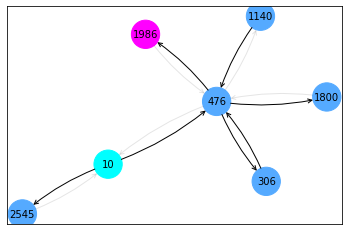
\includegraphics[width=\textwidth]{gnn_exp} 
        \caption{GNN Explainer}
    \end{minipage}\hfill
    \begin{minipage}{0.5\textwidth}
        \centering
        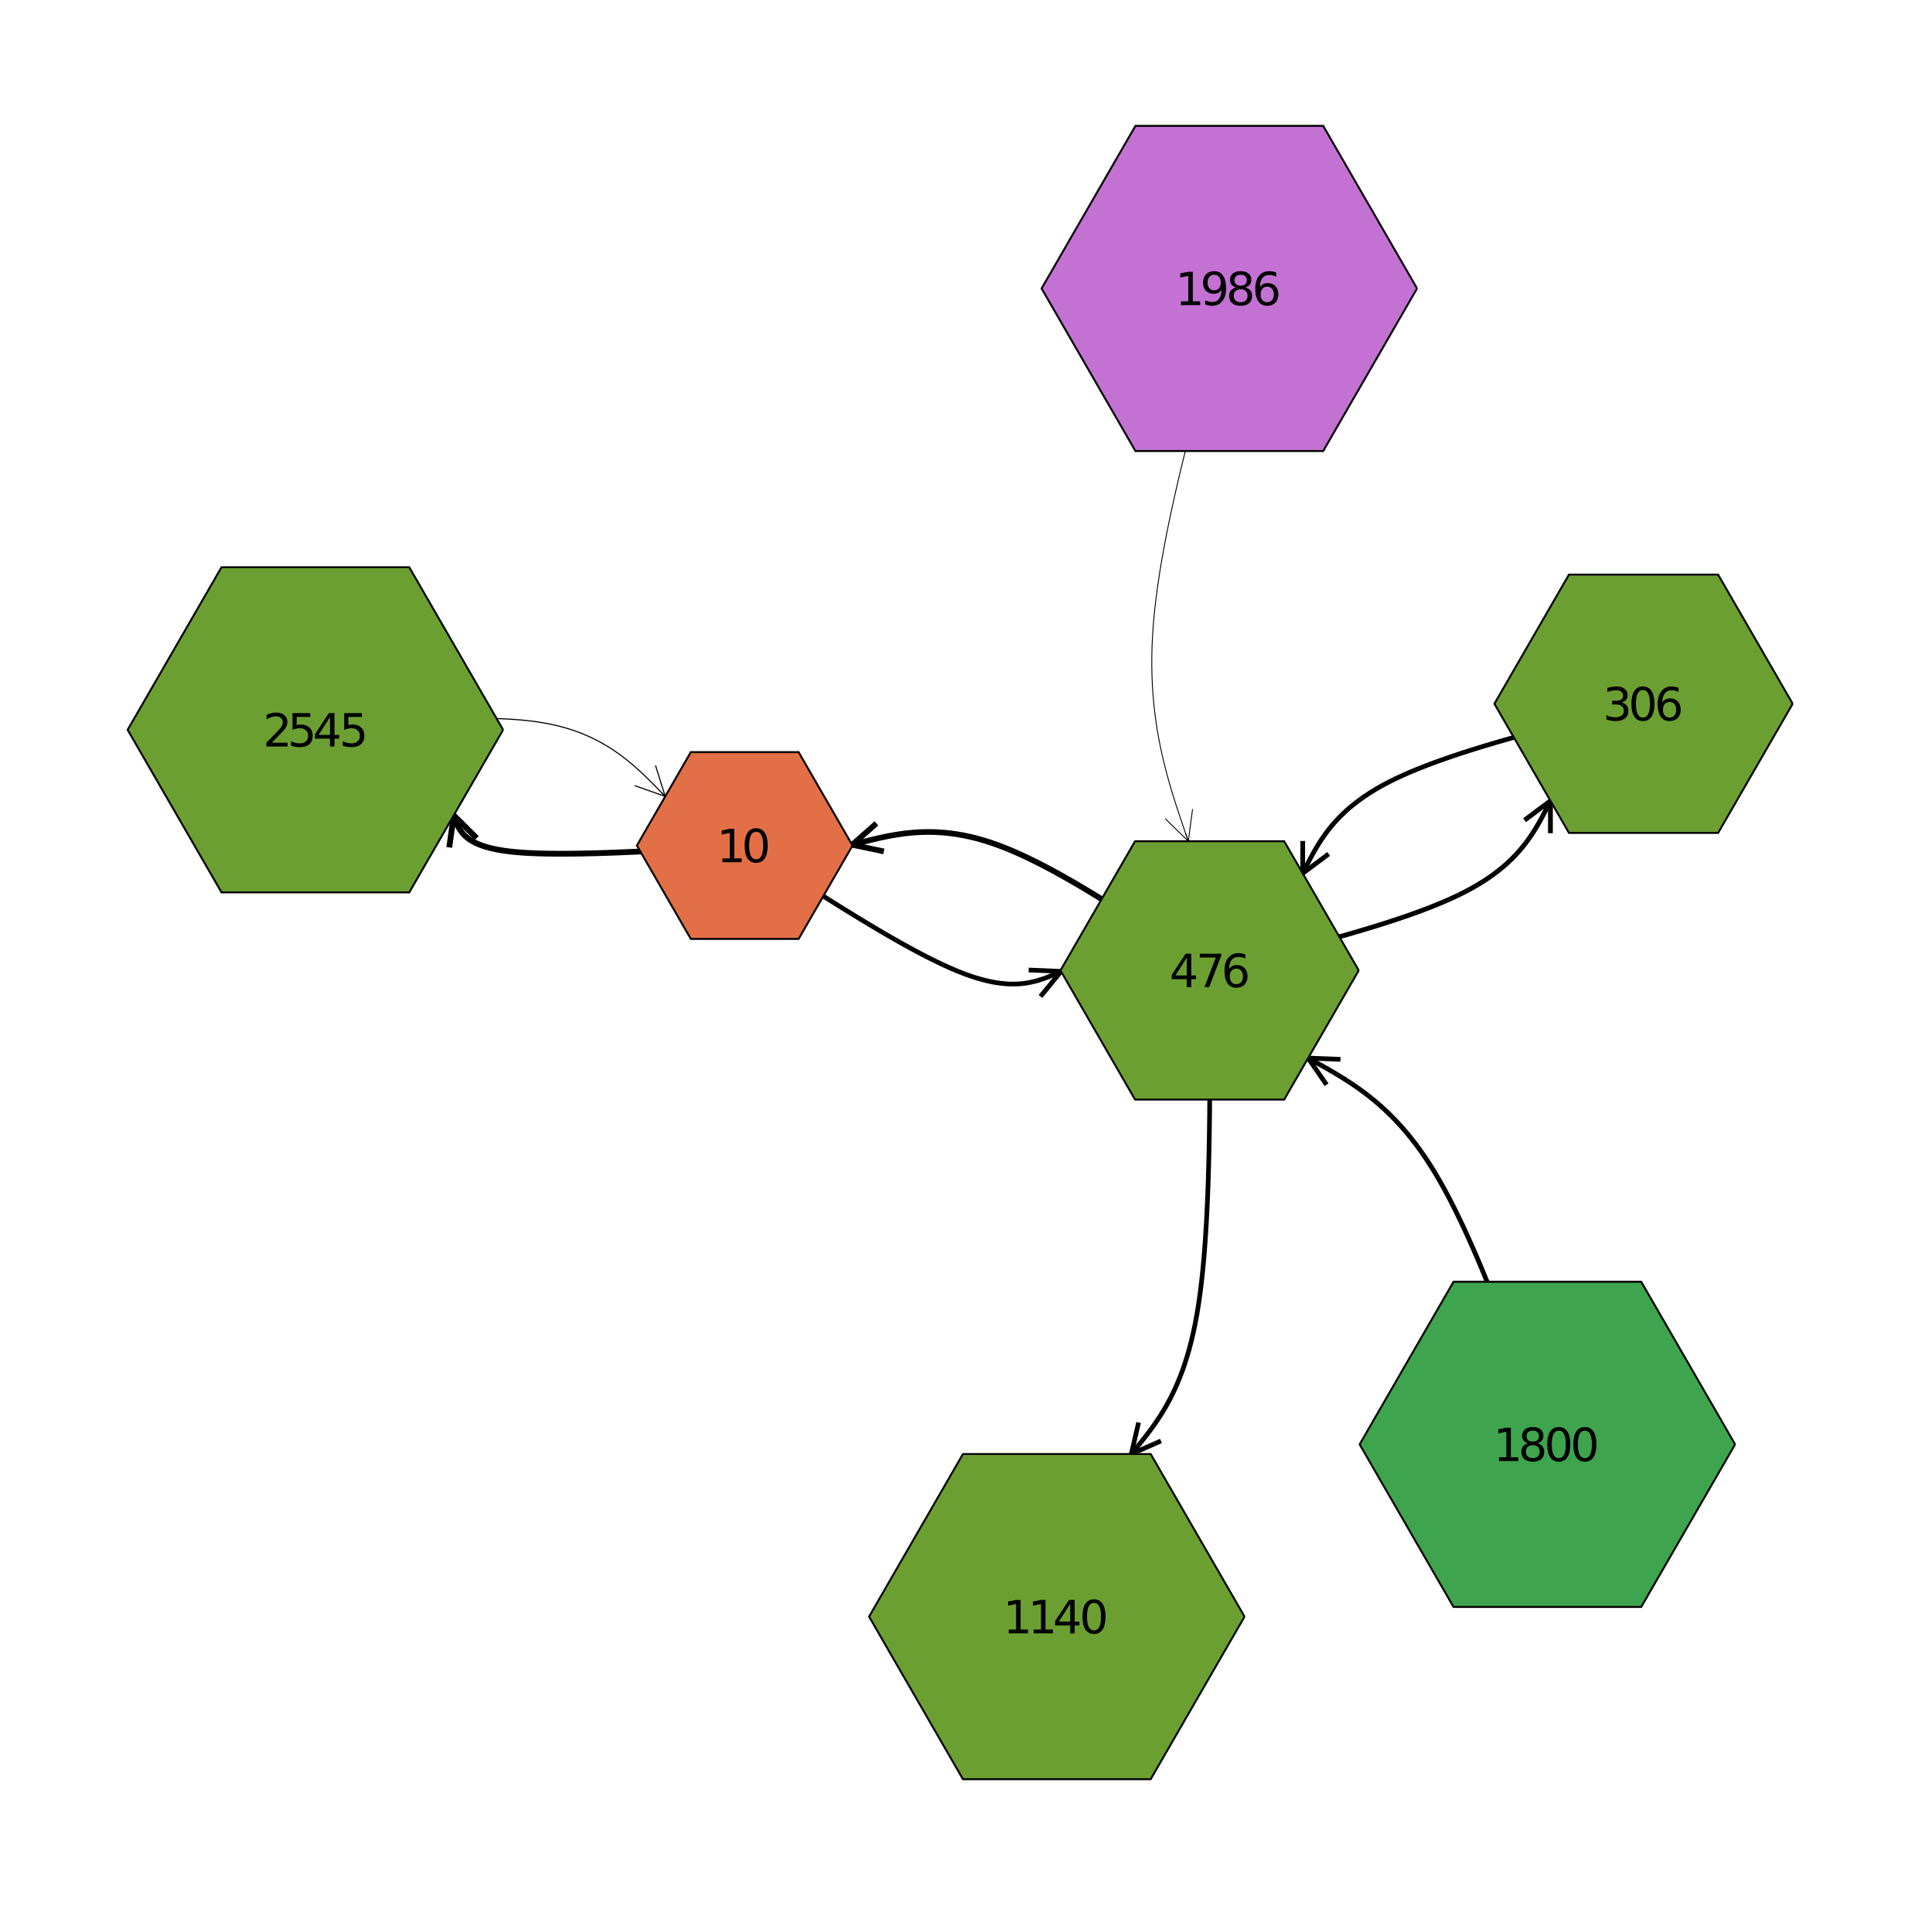
\includegraphics[width=\textwidth]{bayes}
        \caption{Bayesian Method}
    \end{minipage}	
\end{figure}
\end{document}
